\chapter{Materials and Method}
\label{cha:materials_and_method}

\section{Dataset}
\label{sec:dataset}

\subsection{Generation}
\label{subsec:generation}

We created our used dataset from approximately 3000 scientific articles in PDF format. An important point was that these articles contained various information, and thereby we ensured that they come from different scientific fields. To be able to use the data we had to separate them from the PDFs and add additional information first.

We used a text mining pre-processing technique as introduced by Vijayarani et al.~\cite{Vijayarani2015} to separate the data from the PDF. This technique consists of three key steps, which are called the extraction-, the stopwords removal-, and the stemming-step. At first we separated the article structure, and the raw text from the PDF. For those we used a framework described in \Cref{subsec:extract_document_structure}. The stopwords removal-, and the stemming step was done as described in \cref{subsec:stop_words} and \Cref{subsec:stemming}.

\begin{table}[!b]
  \centering
  \begin{tabular}{C{2.6cm} C{2.7cm} C{1.5cm} C{1.5cm} C{1.5cm} C{1.5cm}}
    \toprule
    & \multicolumn{3}{c}{\textbf{per Section Title}} & \multicolumn{2}{c}{\textbf{Overall}} \\
    \textbf{IMRaD Type} & \textbf{Section Title} & \textbf{\# Paper} & \textbf{Percent} & \textbf{\# Paper} & \textbf{Percent} \\ \midrule
    Introduction & Introduction & $822$ & $100\%$ & $822$ & $100\%$ \\ \midrule
    Related Work & Related Work & $465$ & $56.57\%$ & $465$ & $56.57\%$ \\ \midrule
    \multirow{3}{*}{Methods} & Method & $97$ & $11.8\%$ & \multirow{3}{*}{$312$} & \multirow{3}{*}{$37.96\%$} \\
    & Model & 134 & $16.3\%$ \\
    & Approach & 81 & $9.85\%$ \\ \midrule
    \multirow{3}{*}{Result} & Experience & $396$ & $48.18\%$ & \multirow{3}{*}{$687$} & \multirow{3}{*}{$83.58\%$} \\
    & Result & 163 & $19.83\%$ \\
    & Evaluation & 128 & $15.57\%$ \\ \midrule
    \multirow{3}{*}{Discussion} & Conclusion & $581$ & $70.68\%$ & \multirow{3}{*}{$773$} & \multirow{3}{*}{$94.04\%$} \\
    & Discussion & 179 & $21.78\%$ \\
    & Future Work & 13 & $1.58\%$ \\
    \bottomrule
  \end{tabular}
  \caption[Mapping of the Section Titles to IMRAD-Types]{\textbf{Mapping of the Section Titles to IMRAD-Types.} This Table shows which section titles was used to generate the IMRaD structure information. Additionally the relation between those titles, and how often they occurs in the used dataset is displayed.}
  \label{tbl:mapping_section_names}
\end{table}

One of the additional details we had to add was IMRaD structure information. The IMRaD structure provides related work to be part of the introduction. Since most of our papers had an own section titled related work we chose to add an additional type for it. We were able to classify the IMRaD structure with simple keyword detection in the section titles. \Cref{tbl:mapping_section_names} shows the mapping between IMRAD-Types and these titles. Because it was not really possible to identify method sections by using the section titles we used information about their position in the article. We manage that by using the related work as upper bound, and the result as lower bound. We classifying all sections between these two bounds as a method section. If the related work section was not available we use the introduction section as upper bound, or if the result section was not available we use the discussion section as lower bound. If one of the two bounds could not be set, we discarded the scientific article. Chapters can have several IMRaD-Types. For example if a section was titled \textit{"Results and Discussion"} it belongs to the types result and discussion.

Another additional details we had to add was links between the scientific articles. For this we performed a semi-automated annotation. Thereby similarities about the references of an article and the titles of all other articles are compared as described in \Cref{sec:text_similarities}, and if they exceed a given threshold a recommendation to create a link between those two was given.

We created each data record in such a way that it can be transferred directly to the database schema shown in \Cref{fig:database_schema}. To reduce noise during the evaluation we removed all articles without any connection to other articles. Finally we had 821 scientific articles in our dataset.

\myfig{database_schema}
      {width=0.70\textwidth}
      {Database Schema for the used Dataset}
      {Database Schema for the used Dataset}
      {fig:database_schema}

\subsection{Structure of a Scientific Article}
\label{sec:structure_scientific_article}

When looking at the scientific article in the database schema in \Cref{fig:database_schema} there are various member attributes. The first important point is that all text values are available raw and processed. The term raw stands for the text being saved as it was separated. Processed text is the raw text after the stopword removal-, and the stemming step.

The author text attribute contains the names and email addresses of all authors. Thereby this attribute has three values. The complete text, the text reduced to emails, and a list of all authors. This part of the article is the only one that is not preprocessed.

\myfig{scientific_articles_tree}
      {width=0.90\textwidth}
      {\textbf{Scientific Article Tree.} In this figure we highlight the hierarchical structure of an typical scientific article. For example it can be composed into multiple sections.}
      {Scientific Article represented as a Tree}
      {fig:scientific_articles_tree}

One of the most important characteristics are the sections, and the underlying structure that comes with it. \Cref{fig:scientific_articles_tree} shows that scientific articles are structured like a tree. It is easy to see that the chapters are non-leaf nodes, and text areas are the leaf nodes. This is reflected in database schema with two lists. One for the subsections, and one for text areas. In addition to the lists, each section itself has a section type. This attribute reflects whether the section is a section, subsection, or subsubsection. The IMRaD structure information is stored as the IMRaD-Type. As described in \Cref{subsec:generation}, each section can have several IMRaD-Types. Each type of section holds its own list of these types. This means that subsections and subsubsections keeps the same IMRaD-Types as the parent section.

We stored word histograms for the article, and the sections so we do not have to discover the complete text for each search request. These histograms contain the term frequencies of the underlying area. So the subsubsections contain the frequencies of their text areas, the subsections contain the frequencies of their text areas, and their subsubsections text areas, and so on. Finally the article holds all term frequencies of the whole document.

The last two attributes of the article are the reference-, and the cited-by-list. If an id is set in the reference, the referenced paper has an entry in the cited-by-list. Additional we stored the text of whole reference, the authors, and other available information like publisher, pages, volume, etc.

\subsection{Citation Network}
\label{sec:citation_network}

\myfig{dataset_generall}
      {width=0.50\textwidth}
      {\textbf{General Structure of a Citation Network.} The timeline indicates that new articles citing existing articles, and thus there can not be cyclic dependencies.}
      {General Structure of a Citation Network}
      {fig:structure_citation_network}

A Citation networks represents the relationship between scientific articles. \Cref{fig:structure_citation_network} shows the structure of such a network. Scientific articles are nodes, and citations are directed edges between these nodes. The timeline indicates that new articles citing existing articles, and thus there can not be cyclic dependencies. ~\cite{kas2011} defined the basic properties of citation networks in their work. In our case the most important ones are:

\begin{itemize}
  \item Directed.
  \item Acyclic.
  \item All edges point backwards in time
  \item Edges are permanent
  \item The existing part is mostly constant. Only the leading edges changes
\end{itemize}

The network is directed and acyclic because each article has a unique publication date and can only cite previously published articles. Due to these properties edges can only point back in time. The edges of the network have to be permanent because the references of the existing articles never changes. When a new node is added it generates edges to existing articles. This means that all other nodes and edges stays constant.

\begin{table}[!b]
  \centering
  \begin{tabular}{ l c }
    \toprule
    \textbf{Number of Nodes}      & $821$  \\ \midrule
    \textbf{Number of Edges}      & $1,716$ \\ \midrule
    \textbf{Number of Cycles}     & $0$    \\ \midrule
    \textbf{Longest Path Length}  & $12$   \\ \midrule
    \textbf{Number of Root Nodes} & $107$  \\
    \bottomrule
  \end{tabular}
  \caption[General Properties about the citation network]{\textbf{General Properties about the citation network.} The citation network represents the relationship between our used scientific articles. The number of nodes indicates the number of articles, and the number of edges citations between those articles. There are no cycles inside the graph, and the longest citation chain consists of 12 articles. There are 107 articles which has no outgoing edges. That means that none of their referred articles are part of our dataset.}
  \label{tbl:general_properties_about_the_graph}
\end{table}

The main properties of our citation network are shown in \Cref{tbl:general_properties_about_the_graph}. Scientific articles are the nodes, and citations are the edges between these nodes. This means that our network consists of 821 articles, and 1,716 citations between these articles. As described in \Cref{fig:structure_citation_network} and the associated timeline there can not be circles inside the graph. During the generation of our dataset we found an exception via preprints, where circles can appear and have to be handled. Preprints are versions of scientific articles which are not peer reviewed, and published in a scientific journal. In our case we removed all preprints from the dataset. The longest path length indicates that the longest citation chain of our network consists of 12 articles. The root nodes are nodes without any outgoing edges. In our network are 107 articles which cite no other article, which means that none of their referred articles are part of our dataset.

\begin{figure}[!t]
  \begin{minipage}{\textwidth}
    \begin{minipage}[b]{0.39\textwidth}
      \centering
      \begin{tabular}{ l c }
        \toprule
        \textbf{Max Degree}    & $98$     \\ \midrule
        \textbf{Mean Degree}   & $5.8767$ \\ \midrule
        \textbf{Median Degree} & $2$      \\
        \bottomrule
    \end{tabular} \\
    \vspace*{1cm}
    (a) Properties
  \end{minipage}
  \begin{minipage}[b]{0.59\textwidth}
    \centering
    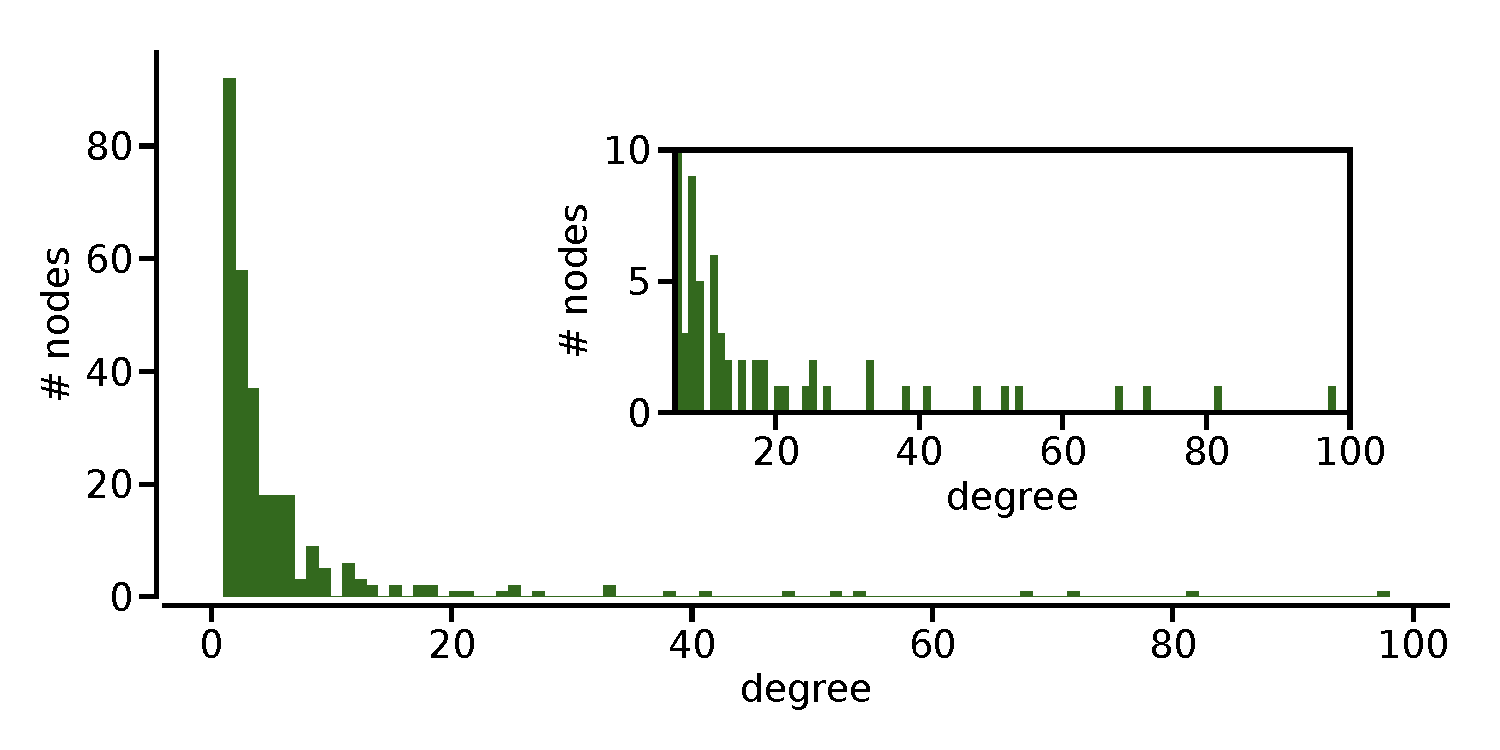
\includegraphics[width=1.0\textwidth]{figures/in-degree_distribution} \\
    (b) In-Degree Distribution
    \end{minipage}
  \end{minipage}
  \caption[In-Degree Distribution of the Citation Network]{\textbf{In-Degree Distribution.} The in-degree distribution describes how often articles get referred by other articles. The positive screw of the distribution indicates that there are a lot of articles which are referred only a few times, and a few articles which are referred more often. There are some single outliers with a higher degree than 20. This can also be seen by the difference between the mean and the median. The max degree in connection with the zoomed view represents that one single article was cited by 98 other articles.}
  \label{fig:indegree_distribution}
\end{figure}

In \Cref{fig:indegree_distribution} the in-degree distribution of our citation network is shown. In general the in-degree of a node is described by the number of ingoing edges. The in-degree distribution represents the probability distribution of these nodes over the whole network. Regarding a citation network the in-degree of a node can be described as the number of articles which referred this article. The positive screw of the in-degree distribution indicates that there are a lot of articles which are referred only a few times, and a few articles which are referred more often. There are only some single articles with an in-degree higher than 20. This is the reason why the median is higher than the mean. The max degree in connection with the zoomed view represents that one single article was referred by 98 other articles.

\begin{figure}[!t]
  \begin{minipage}[!t]{\textwidth}
    \begin{minipage}[b]{0.39\textwidth}
      \centering
      \begin{tabular}{ l c }
        \toprule
        \textbf{Max Degree}    & $13$     \\ \midrule
        \textbf{Mean Degree}   & $2.4034$ \\ \midrule
        \textbf{Median Degree} & $2$      \\
        \bottomrule
    \end{tabular} \\
    \vspace*{1cm}
    (a) Properties
  \end{minipage}
  \begin{minipage}[b]{0.59\textwidth}
    \centering
    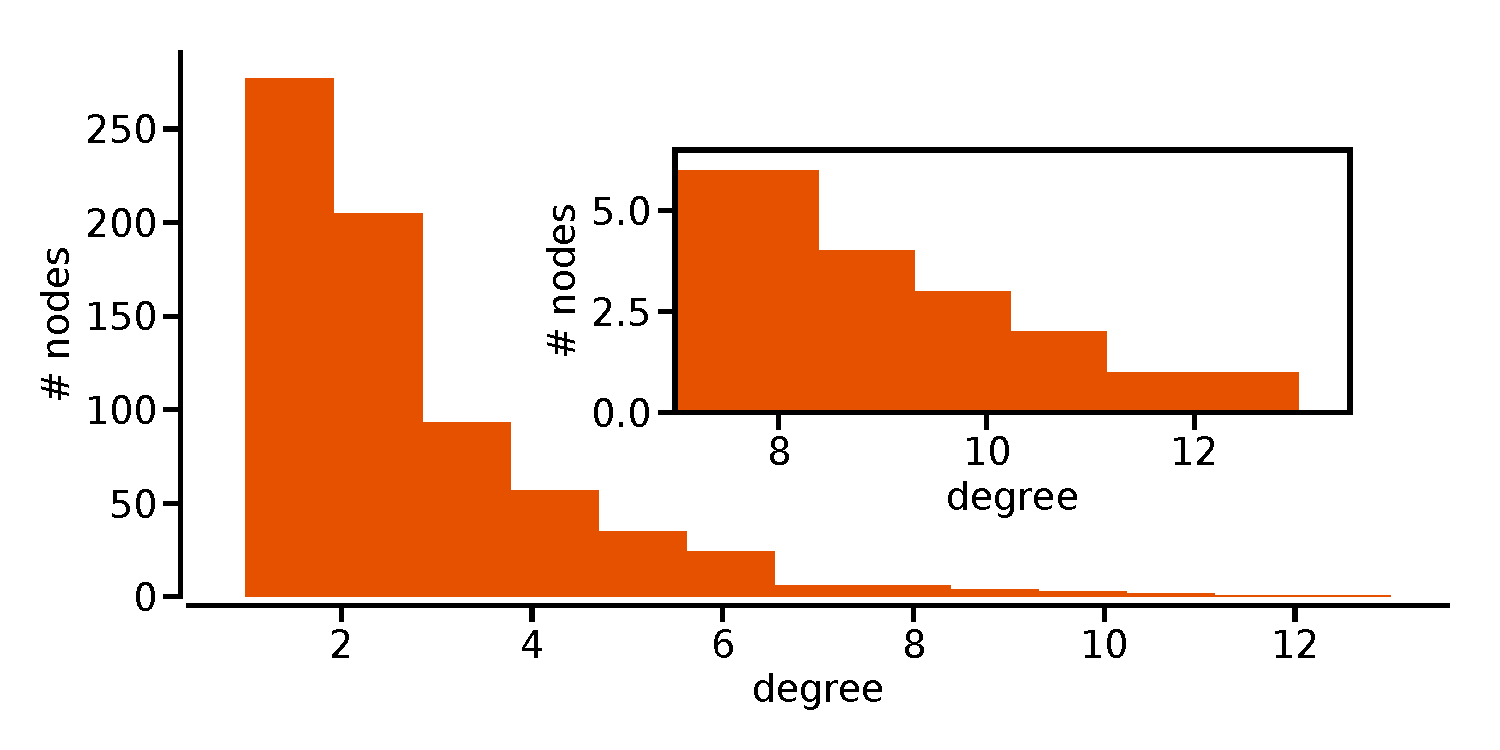
\includegraphics[width=1.0\textwidth]{figures/out-degree_distribution} \\
    (b) Out-Degree Distribution
    \end{minipage}
  \end{minipage}
\caption[Out-Degree Distribution of the Citation Network]{\textbf{Out-Degree Distribution.} The out-degree distribution describes how often articles refer other articles. The positive screw of the distribution indicates that there are a lot of articles which refer less than 7 other articles, and only few with refer to more articles. This number is less because not every referred article is part of our dataset. By the small distance between the mean and the median can be seen that there are less outliers. The max degree represent that the maximum number of a single article refer other articles is 13.}
\label{fig:outdegree_distribution}
\end{figure}

The out-degree distribution and their properties are displayed in \Cref{fig:outdegree_distribution}. Different to the in-degree distribution describes the out-degree distribution the number of outgoing edges. Regarding to the citation network the out-degree of a node can be described as the number of articles which gets referred by this article. The positive screw of the out-degree distribution indicates that there are a lot of articles which refer less than 7 other articles, and only few with refer 7 or more articles. In general articles contains more than 7 references. The mean and median of the outgoing edges are lower, because not every article is part of our dataset. By the small distance between the mean and the median can also be seen that there are less outliers. The max degree represent that the maximum number of a single article refer other articles is 13.

\section{Model}
\label{sec:model}

Write general about information retrieval models as described in ~\cite{ModernInvormationRetrieval1999} page 57

\subsection{Query Structure}

Write how a query looks like - explicit and implicit

\subsection{Introducing IMRaD Structure Features into Weighing Schemes}

Write how the algorithms described in \cref{sec:ranking_algorithms} are modified for imrad structure features.
